\section{Data Pre-processing}
The dataset used in this study is sourced from a CSV file containing detailed specifications of Intel CPUs. This dataset serves as the foundation for our analysis, providing a comprehensive overview of various CPU features necessary for predicting prices. In this section, we describe the structure and contents of the dataset, including the types of features available and their relevance to our study.

\subsection{Dataset Overview}
The CSV file comprises numerous rows, each representing an individual Intel CPU model. Each row contains multiple attributes that describe the specifications and characteristics of the CPU. The dataset includes a diverse range of CPU models, spanning different series, generations, and intended applications (e.g., consumer desktops, laptops, and server-grade CPUs). This diversity ensures that our analysis covers a broad spectrum of CPU types and their respective price points.

\subsection{Data Relevance and Usefulness}

The attributes in the dataset are crucial for predicting CPU prices because they encapsulate the key characteristics that drive market value. Below, we elaborate on the significance of each attribute in influencing CPU pricing:

\begin{itemize}
    \item \textbf{Clock Speed}: Measured in gigahertz (GHz), clock speed is a primary performance indicator. CPUs with higher clock speeds can execute more instructions per second, thus enhancing overall performance. This makes clock speed a pivotal factor in pricing, as consumers and professionals often seek higher clock speeds for better performance.
    
    \item \textbf{Number of Cores}: The number of cores in a CPU affects its ability to handle multiple tasks simultaneously. Multi-core CPUs can manage parallel processes more efficiently, which is especially beneficial for tasks such as video editing, gaming, and running multiple applications. As a result, CPUs with more cores generally command higher prices.
    
    \item \textbf{Number of Threads}: Threads are the smallest units of processing that the operating system can schedule. CPUs with more threads can improve parallel processing capabilities, contributing to better multitasking and performance in threaded applications. This attribute is directly correlated with pricing, as higher thread counts enhance performance.
    
    \item \textbf{Cache Size}: Cache memory, typically measured in megabytes (MB), stores frequently accessed data for quick retrieval. Larger cache sizes reduce latency and improve processing speed, making CPUs with substantial cache memory more desirable and thus more expensive.
    
    \item \textbf{Power Consumption}: Measured in watts (W), power consumption impacts the efficiency and thermal performance of a CPU. CPUs that offer high performance while maintaining lower power consumption are more attractive, particularly for mobile devices and energy-efficient systems. Efficient power consumption can justify higher prices due to lower operating costs and reduced cooling requirements.
    
    \item \textbf{TDP (Thermal Design Power)}: TDP indicates the amount of heat a CPU generates under typical load conditions. CPUs with lower TDP values can be easier to cool, which is a significant consideration for system builders looking to manage heat dissipation effectively. This can influence the price, as better thermal performance can be a premium feature.
    
    \item \textbf{Manufacturing Process}: The technology node (e.g., 14nm, 10nm) used in manufacturing a CPU affects its performance, power efficiency, and cost. Smaller manufacturing processes generally lead to more efficient and powerful CPUs, contributing to higher prices due to the advanced technology involved.
    
    \item \textbf{Release Date}: The release date provides context regarding the technological advancements and market conditions at the time of a CPU's launch. Newer CPUs often incorporate the latest technologies and improvements, justifying higher prices compared to older models.
\end{itemize}

Our objective is to develop predictive models that can accurately estimate the price of a CPU based on its specifications. Understanding the relationship between each attribute and the price is essential for creating effective models. For instance, clock speed, core count, and cache size are direct performance indicators, while power consumption and TDP relate to efficiency and usability in different environments. The manufacturing process and release date provide context about the technological and market influences on pricing.\\

By focusing on these critical attributes, we aim to develop models that capture the complexities of CPU pricing. This will enable us to make accurate predictions and provide valuable insights for manufacturers and consumers in the decision-making process.

\subsection{Load Data}
\begin{lstlisting}[language=R]
    # Importing data 
    intel_cpu <- read.csv ("~/Downloads/archive/Intel_CPUs.csv")
\end{lstlisting}

This line of R code is used to import a dataset from a Comma-Separated Values (CSV) file into the R environment.
The \texttt{read.csv()} function is a built-in function in R that reads a CSV file and creates a data frame object from its contents. A data frame is a two-dimensional tabular data structure in \texttt{R}, where each column represents a variable, and each row represents an observation.\\

In this specific code:
"\textbf{$\sim$/Downloads/archive/Intel\_CPUs.csv}" is the file path that specifies the location and name of the CSV file to be imported, \texttt{intel\_cpu} is the name assigned to the data frame object that will store the imported data.\\

After executing this line of code, the contents of the "\textbf{Intel\_CPUs.csv}" file will be read and stored in the \texttt{intel\_cpu} data frame within the \texttt{R} environment. The data frame will have the same structure as the CSV file, with columns representing variables and rows representing observations.

\subsection{Explore Data}
\begin{lstlisting}[language=R]
    # The head () function is used to preview the first 
    # few rows of the data frame
    head (intel_cpu)
\end{lstlisting}

This line calls the \texttt{head()} function and passes the \texttt{intel\_cpu} data frame as an argument. By default, the \texttt{head()} function prints the first \textit{six} rows of the given data frame or matrix.\\

The \texttt{head()} function is a valuable tool for data exploration and validation, especially when working with large datasets. By previewing the initial rows, you can quickly assess the structure of the data, check the column names, and ensure that the data has been imported correctly.\\

Inspecting the first few rows can reveal potential issues or anomalies in the data, such as missing values, incorrect data types, or unexpected values. It also provides an initial glimpse into the content and format of the data, which can inform subsequent data cleaning, transformation, or analysis steps

\begin{figure}[H]
    \centering
    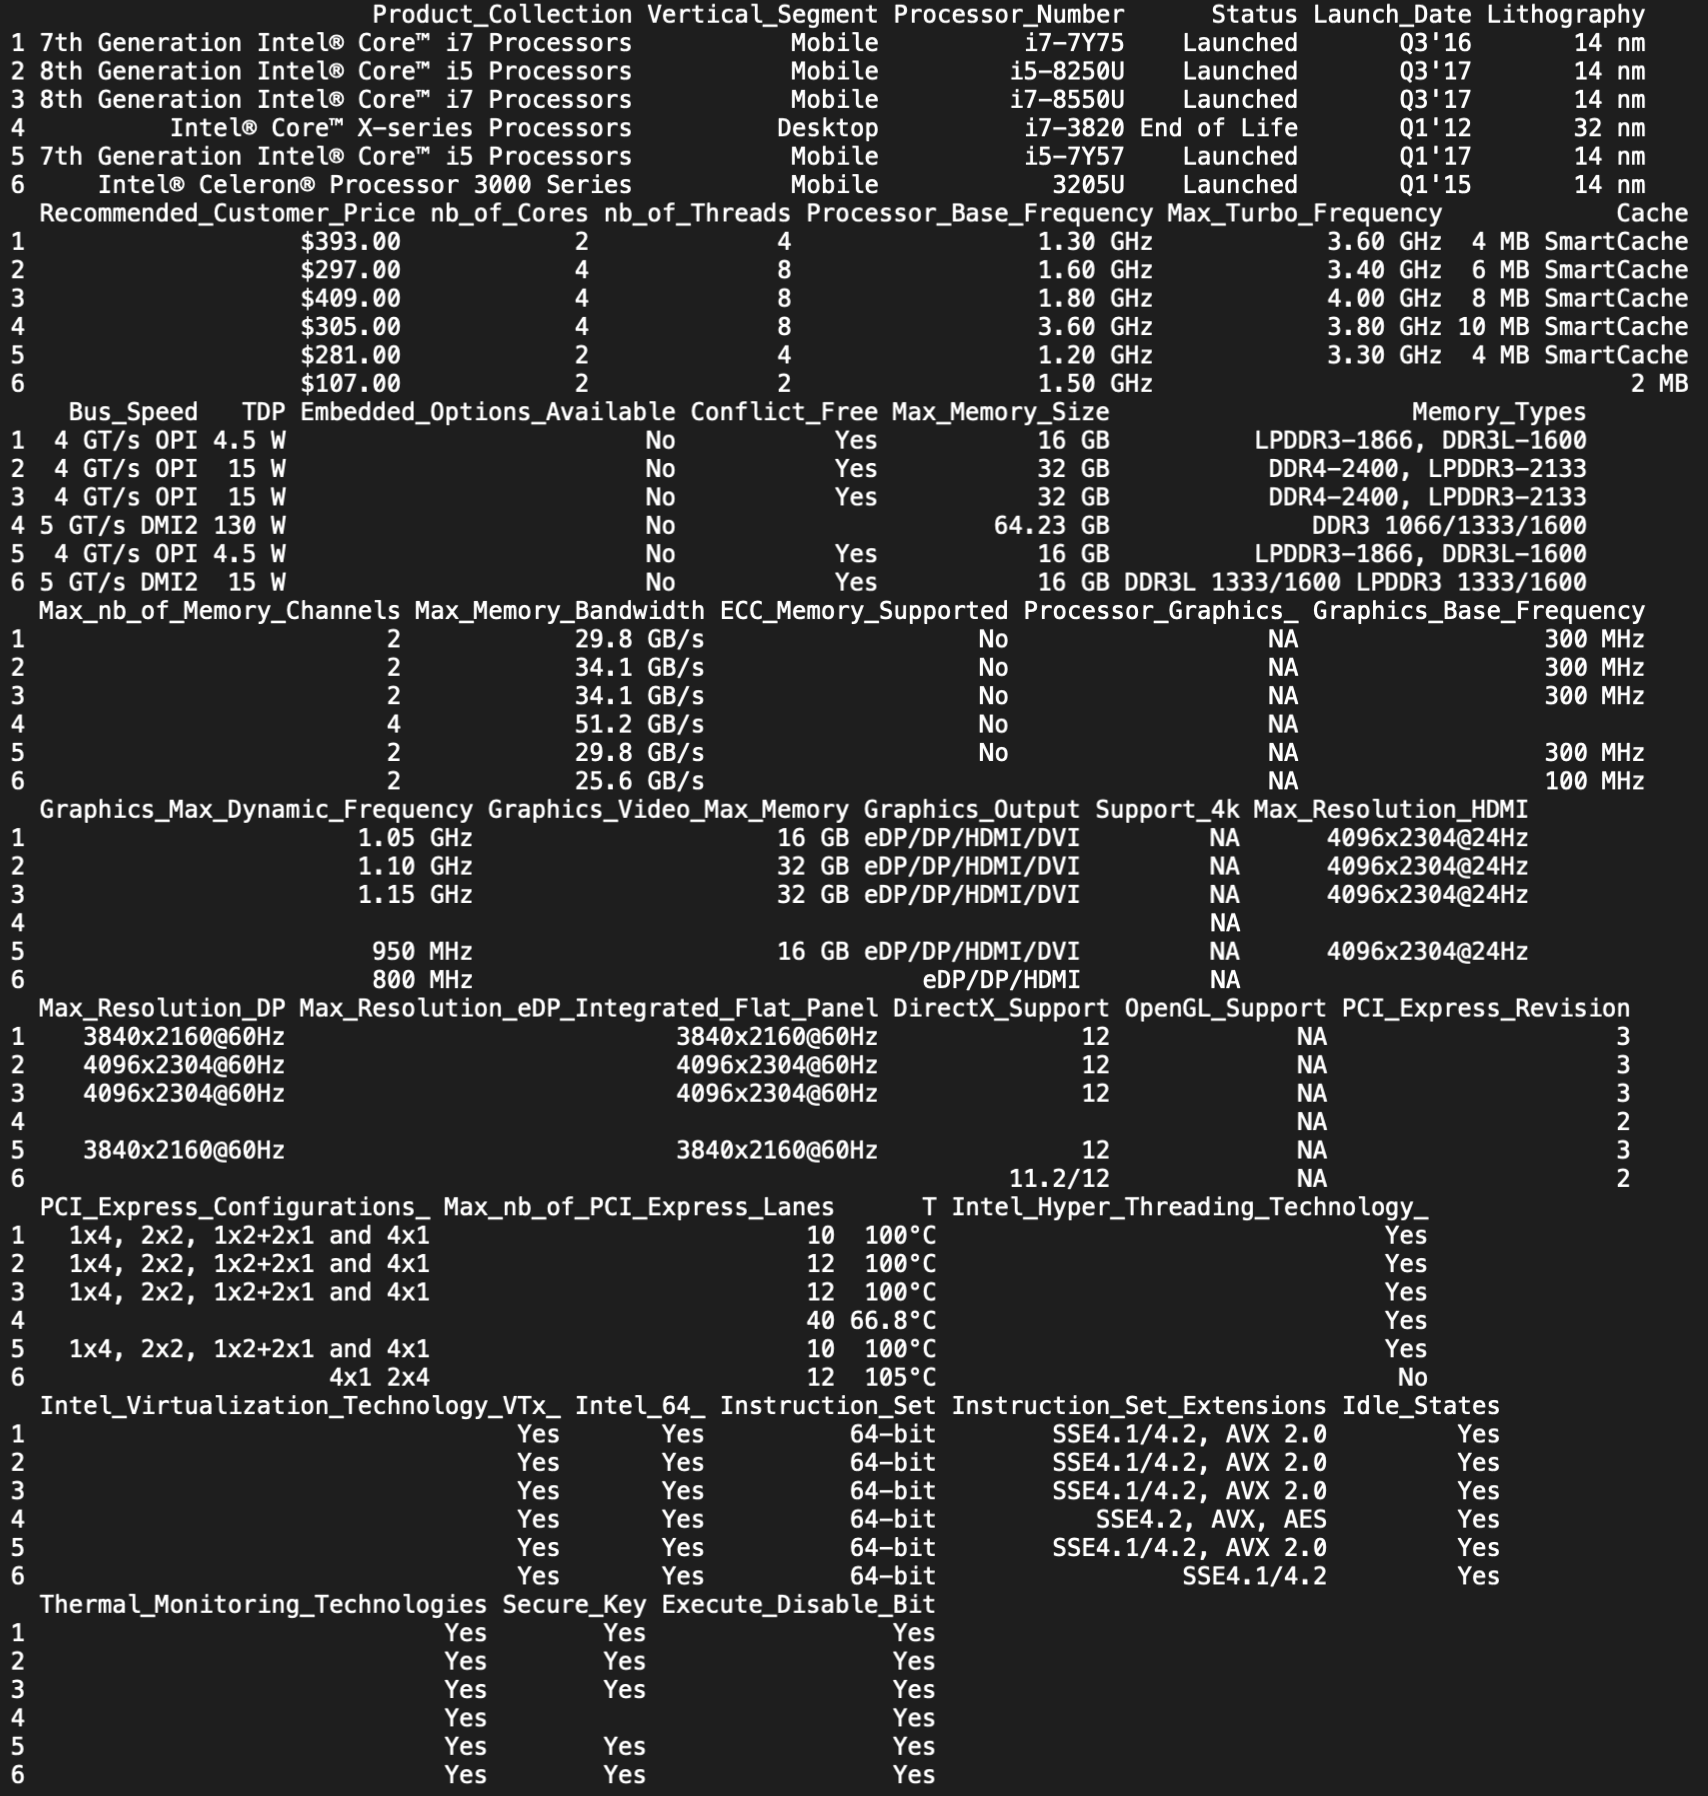
\includegraphics[width=14cm]{graphics/head.png}
    \caption*{Console output of \texttt{head(intel\_cpu)}}
\end{figure}

By executing \texttt{head(intel\_cpu)}, the output will display the first \textit{six} rows of the \texttt{intel\_cpu} data frame, allowing you to visually inspect the data and make informed decisions about the next steps in the data analysis workflow.

\newpage

\begin{lstlisting}[language=R]
    # Summary statistics
    summary (intel_cpu)
\end{lstlisting}

This code snippet is used to obtain summary statistics for the dataset stored in \texttt{intel\_cpu}.\\

The \texttt{summary ()} function in \texttt{R} is a versatile tool that provides a consise summary of the data, depending on the type of input it receives.

\begin{figure}[H]
    \centering
    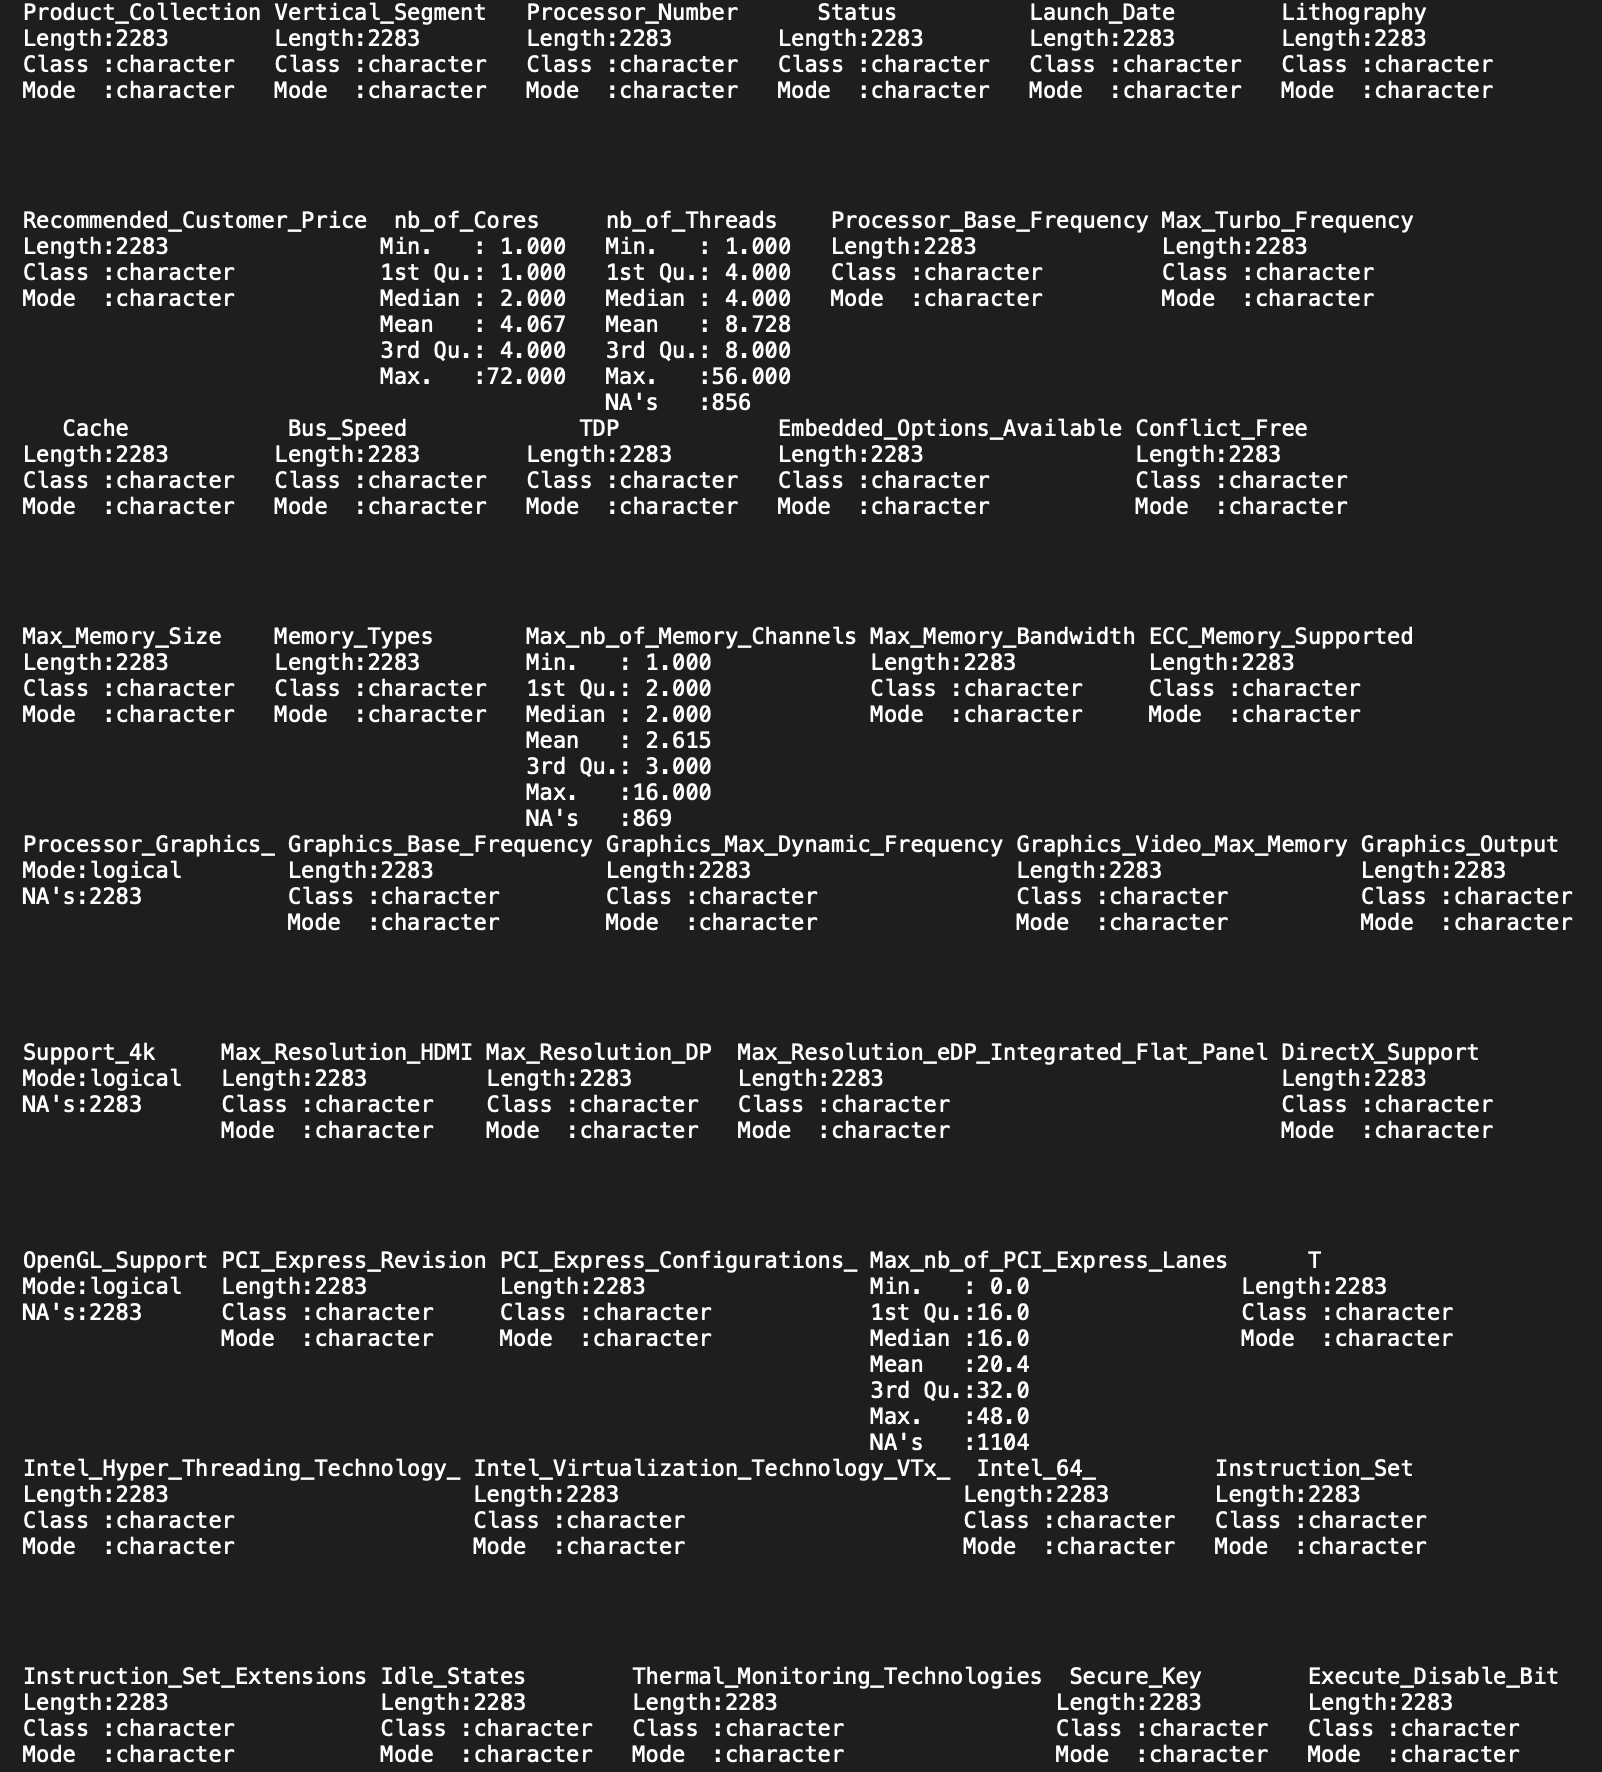
\includegraphics[width=14cm]{graphics/summary.png}
    \caption*{Console output of \texttt{summary(intel\_cpu)}}
\end{figure}

\subsection{Handle Missing Values}

\subsection{Handle Outliers}

\subsection{Feature Scaling/Normalization}

\newpage